\documentclass[11pt]{article}
\usepackage{fancyhdr}
\usepackage{times}
\usepackage{graphicx}
\usepackage{hyperref}
\usepackage[a4paper,top=3.5cm,left=3.5cm,right=3.5cm,bottom=3cm]{geometry}

\title{\textsf{FIRMAMENT}\\ Operation Manual}
\date{Version 1.0}
\author{Roberto Jung Drebes}

\fancyhead[R]{
\includegraphics[scale=0.25]{fig/firmament.png}}
\fancyhead[L]{\textsf{FIRMAMENT} \\ {\em Operation Manual}}


\begin{document}

\pagestyle{fancy}

\maketitle

\section{Introduction}


This manual presents \textsf{FIRMAMENT}'s specification and details its operation: the faultlet concept, instructions recognized by the tool's virtual machine and the supported control commands. This document is a starting point for people interested in testing network protocols and aplications using \textsf{FIRMAMENT}.

\section{Faultlets}\label{sec:faultlet}

A typical drawback of usual communication fault injectors is the restricted way in which fault scenarios can be specified. The coding of the operations to be performed over messages depends on the possible actions allowed by the tool. The approach ends up being very strict and specific for pre-existing protocols.

Even when it is possible to specify actions based on message content, this is usually limited, since tests can be made on fixed message offsets. The data of a packet cannot be read and used as a parameter for the injector actions, nor processed combinedly to determine such actions.

An example of the inconvenience caused by this limitation is the processing of the IPv4 protocol header. IPv4 has a variable header size. If we would like to inspect its data area, it is not enough to simply jump over a fixed number of initial bytes belonging to the header. It is necessary to read, from the header, its size, and use this information as an index for accessing the packet data area. Making it even more complex, the IPv4 header size is indicated in the number of 32 bit words, so if the header size is wanted in bytes the information should be multiplied by 4.

This complication is not exclusive of IPv4. IPv6, unlike IPv4, has a basic header with a fixed size, but the transport layer header does not always immediately follows the basic header.  Since it uses a chained header structure, the transport layer header is located only after the structure which may contain optional headers, and so faultlet processing should repeatedly verify the following header type until it finds a UDPv6 or TCPv6 header.

Traditional communication fault injectors can be developed considering these issues and by doing so support such protocols, through the previous knowledge about its format. However, this approach is not extensible to new protocols, and limits the test engineer to the scenarios and protocols already supported by the tool. Even if the tool supports the processing of IP headers, the test target can be an application protocol. Although many aplication protocol are documented through RFCs ({\em Request for Comments}), this is not always the case, and so it is complex to develop a generic protocol testing tool using the usual approaches to specify scenarios. 

\textsf{FIRMAMENT} extensibility comes from its new approach for fault scenary specification, through a simple, however flexible, technique. The tool employs the {\em faultlet} concept, a fault aplication whose difference is the power of expression of fault scenarios.

A faultlet is executed over each packet that crosses the communication flows, and it is able to inspect and modify the contents of the packet, discard, duplicate or delay it. In addition to the packet, a faultlet can act over the flow state variables: a set of general purpose registers. It can, therefore, move data between the packet and its state variables, and perform logical, arithmetic and control operations over these data. Hence, the execution flow of a faultlet can be modified by data read from the packet. This is the key characteristic of the tool: the possibility to create advanced control structures, with loops and branches, making \textsf{FIRMAMENT} appropriate to test any protocol.

Faultlets are independently configured for the input and output flows\footnote{The processing of distinct faultlets on receiving and sending allows fault injection associated to assimetric topologies.} of the IPv4 and IPv6 protocol families. A faultlet is executed by the \textsf{FIRMVM} virtual machine, a module of \textsf{FIRMAMENT} connected to the communication subsystem through the Netfilter interface. It is the \textsf{FIRMVM} virtual machine that actually associate a packet to a faultlet and the state variables. The next section describes the \textsf{FIRMVM}, listing the instructions and the state variables available to faultlet programming. 

\section{The \textsf{FIRMVM} virtual machine}\label{sec:instructions}

The \textsf{FIRMVM} virtual machine is the module responsible for interpreting and processing the instructions which specify fault scenarios. \textsf{FIRMVM} works over 4 package flows, associated to the input and output of the IPv4 and IPv6 protocols. The fault scenario specification for these flows is done independently, writing faultlets to the tool's virtual files interface described in Section~\ref{sec:arqvirtuais}. This section presents the state variables  avaliable for faultlets processing as well as the avaliable instructions for building faultlets.

\subsection{State variables}
 
In addition to the contents of the packets, each flow can operate over a set of general purpose registers. The registers are intianted when a flow is started and its state is kept during the sequential processing of all its packets, therefore being able to be used as state variables. 

A set of 16 general purpose 32 bit registers is avaliable for each flow. From the point of view of the faultlet programmer, the registers use a network byte order representation (MSB/BIG\_ENDIAN), i.e, it is in this format data must be read or written to the registers. However, \textsf{FIRMAMENT} does automaticallt convert from the native hardware format to this format. The register specification for the programmer in the \textsf{FIRMASM} language (described next) is always in the form $R_x$, where $x$ is an integer from 0 to 15.

Each register can be configured to be auto-incremented periodically. To each increment is associated a wake up period, in millisenconds, and the register is incremented when this period is reached. Instructions allow the activation and deactivation of the auto-increment individually for each register. Increment precision dependends on the timing resolution of the platform's timer interrupt, tipically between 1 and 10 ms.

\subsection{Instructions}

Faultlets are specified using a group of 29 instructions organized in 7 classes. The instructions have a textual representation, called \textsf{FIRMASM}, used by the assembler \texttt{firm\_asm} presented in Section~\ref{sec:firmasm}. The instruction set and its textual representation are listed below.

\subsubsection{Input and output instructions}

\begin{itemize}
 
\item \textbf{\texttt{READB Ry  Rx} (Read byte from packet)} 

Reads in $R_x$ the contents of the byte of the packet pointed by $R_y$ (in bytes). If the content of $R_y$ is greater than the length of the packet in bytes, the value of $R_x$ is not modified.

$R_x \leftarrow \mbox{(8 bits) packet[$R_y$]}$


\item \textbf{\texttt{READS Ry  Rx} (Read short from packet)}

Reads in $R_x$ the contents of the short (16 bits) of the packet pointed by $R_y$ (in bytes). If the content of $R_y$ is greater than the length of the packet in bytes (minus one, to leave room for the remaining byte), the value of $R_x$ is not modified.

$R_x \leftarrow \mbox{(16 bits) packet[$R_y$]}$


\item \textbf{\texttt{READW Ry  Rx} (Read word from packet)} 

Reads in $R_x$ the contents of the word (32 bits) of the packet pointed by $R_y$ (in bytes). If the content of $R_y$ is greater than the length of the packet in bytes (minus three, to leave room for the remaining bytes), the value of $R_x$ is not modified.

$R_x \leftarrow \mbox{(32 bits) packet[$R_y$]}$


\item \textbf{\texttt{WRTEB Ry  Rx} (Write byte to packet)} 

Writes to the byte of the packet pointed (in bytes) by $R_y$ the contents of the least significant byte of register $R_x$. If the content of $R_y$ is greater than the length of the packet in bytes, the instruction has no effect.

$\mbox{packet[$R_y$]} \leftarrow \mbox{(8 bits)\ } R_x$

\item \textbf{\texttt{WRTES Ry  Rx} (Write short to packet)}

Writes to the short (16 bits) of the packet pointed (in bytes) by $R_y$ the contents of the least significant short of register $R_x$. If the content of $R_y$ is greater than the length of the packet in bytes(minus one, to leave room for the remaining byte), the instruction has no effect.

$\mbox{packet[$R_y$]} \leftarrow \mbox{(16 bits)\ } R_x$


\item \textbf{\texttt{WRTEW Ry  Rx} (Write word to packet)} 


Writes to the word (32 bits) of the packet pointed (in bytes) by $R_y$ the contents of the register $R_x$. If the content of $R_y$ is greater than the length of the packet in bytes (minus 3, to leave room for the remaining bytes), the instruction has no effect.

$\mbox{packet[$R_y$]} \leftarrow \mbox{(32 bits)\ } R_x$

\item \textbf{\texttt{SET y  Rx} (Set a value into a register)} 

Register $R_x$ is set with the absolute value $y$.

$R_x \leftarrow \mbox{(32 bits)\ } y$


\end{itemize}


\subsubsection{Logic and arithimetic instructions}


\begin{itemize}




\item \textbf{\texttt{ADD  Ry  Rx} (Add register)} 

Register $R_x$ receives the value of the arithmetic addition of registers $R_y$ and $R_x$.

$R_x \leftarrow R_x + R_y$


\item \textbf{\texttt{SUB  Ry  Rx} (Subtract register)} 

Register $R_x$ receives the value of the arithmetic subtraction of registers $R_y$ and $R_x$.

$R_x \leftarrow R_x - R_y$

\item \textbf{\texttt{MUL  Ry  Rx} (Multiply register)}

Register $R_x$ receives the value of the arithmetic multiplication of registers $R_y$ and $R_x$. 

$R_x \leftarrow R_x \times R_y$

\item \textbf{\texttt{DIV  Ry  Rx} (Divide register)} 

Register $R_x$ receives the value of the integer arithmetic divison of register $R_x$ by the contents of register $R_y$. 

$R_x \leftarrow R_x \div R_y$


\item \textbf{\texttt{AND  Ry Rx} (``AND'' bitwise register operation)} 

Register $R_x$ receives the value of the ``AND'' bitwise logic operation of registers $R_y$ and $R_x$.

$R_x \leftarrow R_x\ \&\  R_y$


\item \textbf{\texttt{OR  Ry  Rx} (``OR'' bitwise register operation)} 

Register $R_x$ receives the value of the ``OR'' bitwise logic operation of registers $R_y$ and $R_x$.

$R_x \leftarrow R_x\ |\  R_y$

\item \textbf{\texttt{NOT  Rx} (Invert register)}

Register $R_x$ receives the value of the logical bitwise invertion of register $R_x$. 

$R_x \leftarrow \ !\ R_x$

\end{itemize}



\subsubsection{Packet action instructions}

\begin{itemize}

\item \textbf{\texttt{ACP} (Accept packet)} 

Packet is accepted. Faultlet processing is concluded.

\item \textbf{\texttt{DRP} (Drop packet)} 

Packet is dropped. Faultlet processing is concluded.

\item \textbf{\texttt{DUP} (Duplicate packet)} 

Packet is duplicated. Faultlet processing is concluded.

\item \textbf{\texttt{DLY Rx} (Delay packet)}

The packet is delayed for the number of milliseconds given in $R_x$. Faultlet processing is concluded.

\end{itemize}

\subsubsection{Branch instructions}

\begin{itemize}

\item \textbf{\texttt{JMP x} (Unconditional branch)}

Faultlet's execution flow is branched to the instruction located at positon $x$ of the faultlet. 

\item \textbf{\texttt{JMPZ Ry x} (Branch if zero)} 

Faultlet's execution flow is branched to the instruction located at positon $x$ of the faultlet if the content of register $R_y$ is zero. 

\item \textbf{\texttt{JMPN Ry x} (Branch if negative)} 

Faultlet's execution flow is branched to the instruction located at positon $x$ of the faultlet if the content of register $R_y$ is negative. 

\end{itemize}



\subsubsection{Auto-increment manipulation instructions}


\begin{itemize}

\item \textbf{\texttt{AION Rx Ry} (Auto-increment activation)} 


Activates the auto-increment for register $R_y$, which increments it periodically using the content of $R_x$ as a period (in milliseconds).

\item \textbf{\texttt{AIOFF Ry} (Auto-increment deactivation)} 

Deactivates the auto-increment for register $R_y$.

\end{itemize}

\subsubsection{String manipulation instructions}


\begin{itemize}

\item \textbf{\texttt{CSTR Ry Rx "{\em string}"} (Compare string)} 


Compares the content of the packet starting at position indicated in $R_y$ to the string \texttt{string}\footnote{String length is limited to 255 characters.}. The value `1' is written to $R_x$ if they are equal, '0' otherwise.

\item \textbf{\texttt{SSTR Ry "{\em string}"} (Writes string)}


Writes the string \texttt{string} to the packet, from the position indicated in $R_y$ to the end of the packet or of the string, whichever occurs first.

\end{itemize}

\subsubsection{Miscelaneous instructions}

\begin{itemize}

\item \textbf{\texttt{MOV Ry Rx} (Copy register)} 

Register $R_x$ is set with the value stored in $R_y$.

\item \textbf{\texttt{RND Ry Rx} (Random number)}


Register $R_x$ is set with a random value which has a modulo between 0 and the value stored in $R_y$.

$R_x \leftarrow \ z$, such that $-R_y < z < +R_y$

\item \textbf{\texttt{SEED Rx Ry Rz} (Pseudo-random number seed)} 

\textsf{FIRMAMENT} uses an algorithm based on the Tausworthe generators to obtain pseudo-random numbers. The default seed value is chosen automatically, but it can be explicitly expressed using this instruction, indicated through the three registers passed as parameters ($R_x$, $R_y$ e $R_z$).

\item \textbf{\texttt{DBG Rx "{\em string}"} (Debug aid)}

Prints to the event log the \texttt{string} string, using the 
contents of $R_x$ to replace its first occurence of the scape sequence in the \texttt{printf} format (e.g., \texttt{\%d} for a decimal representation, \texttt{\%x} for an hexadecimal representation and so on).

\item \textbf{\texttt{DMP} (Dump packet)} 

Dumps (prints) the full packet contents in hexadecimal form through the system log.

\item \textbf{\texttt{VER Rx} (Virtual machine version)} 

Register $R_x$ is filled with the version number of the running \textsf{FIRMVM} virtual machine. The textual representation of the version number, expressed in the form $A.B$ (where $A$ represents the major version and $B$ the minor), is stored in the register in the form $(A << 16) + B$.

$R_x \leftarrow \mbox{version(\textsf{FIRMVM})} $

\end{itemize}


\section{Watchdog mechanism}


The \textsf{FIRMVM} register machine is {\em Turing-complete}. As such, faultlets executed over it can put the system into an infinite loop, causing the fault injection node to crash. Since it is impossible to avoid this, \textsf{FIRMAMENT} has a mechanism to interrupt such situations, and do not permit the faultlet processing function to freeze.

A watchdog mechanism detects fuctions that take excedingly long to complete, interrupting their execution. In this case, when reaching this time limit the packet is accepted and continues to flow through the protocol stack as is (i.e., if the faultlet alters the packet, these changes are kept). The default timeout of the watchdog mechanism is 20 milliseconds, but it can be modified (or even disabled) through the \texttt{settimeout} control command presented in Section~\ref{sec:arqvirtuais}.

This feature, beyond offering an extra protection to the user regarding the use of ill-constructed faultlets, allows the tool to be used in soft realtime aplications, since it is then possible to limit the tool's maximum intrusiveness through an upper limit to the time it takes to perform the fault injection and packet processing.

\section{\textsf{FIRMASM} assembler}\label{sec:firmasm}


\textsf{FIRMAMENT} does not directly decode the literal form of the instructions presented in Section~\ref{sec:instructions}. Instead, it decodes instruction in a binary format which is more appropriate to be processed in kernel space. This requires a translation, or assembly, of the literal form into the binary format.


\texttt{firm\_asm} is the \textsf{FIRMAMENT} assembler. When invoked, it receives an input file as parameter, which should be described using the \textsf{FIRMASM} language, as well as an optional parameter indicating the output filename. If the second parameter is omitted, the default value of \texttt{fa.out} is assumed. This parameter can indicate directly one of the virtual files existing in the \texttt{/proc/net/firmament/rules} directory, described in the next section, and this prevents the creation of intermediary files.

The assembly utility verifies parameter typing of the instructions, preventing malformed {\em faultlets} from being loaded into the injector. This permits some simplifications to the kernel-internal implementation part of the instruction decoder, which provides savings in complexity and intrusivity during experiment runtime.


The tool also support labels: offset indicators which can be used as parameters to the branch instructions. The definition of a label can contain up to 10 characters, it should always be located before an instruction and finish with `:' character. A reference to the label should ommit this character. Also, both labels as well as instructions are case insensitive.

String manipulation instructions allow the user to indicate non-printable characterers (or any other ASCII character\footnote{Except the null character (code 0). This is a limitation of the assembler, not of the interpreter.}) by its octal or hexadecimal representation by escape sequences. The complete listing of special characters supported can be seen on Table~\ref{tab:escape}.


\begin{table}[htbp]
  \centering
  \caption{String escape codes}
  \begin{tabular}{lp{4cm}lp{4cm}}
    \hline
    \texttt{\textbackslash a} & bell (alert) & \texttt{\textbackslash t} & tab \\
    \texttt{\textbackslash b} & backspace & \texttt{\textbackslash v} & vertical tab \\
    \texttt{\textbackslash f} & form-feed & \texttt{\textbackslash \textbackslash} & backslash \\
    \texttt{\textbackslash n} & new-line & \texttt{\textbackslash {\em ooo}} & octal number \\
    \texttt{\textbackslash r} & carriage return & \texttt{\textbackslash x{\em hh}} & hexadecimal number \\
\texttt{\textbackslash "} & double quote \\
    \hline
  \end{tabular}

  \label{tab:escape}
\end{table}


The instruction which loads absolute values into registers (\texttt{SET}) can interpret hexadecimal or decimal numbers. For hexadecimal representation, numbers must be indicated with a preceeding ``\texttt{0x}'' and always considered unsigned. For decimal, either positive or negative numbers can be used.


Faultlets can be commented using the semicolon charecter (`;') at any point in the input (except inside string sequences, in which case it is considered part of the sequence). All text in the same line following this character is ignored.

There is also a complimentary tool, called \texttt{msa\_mrif}, which allows the conversion the other way, ``unassembling'' faultlets from its binary representation into the mnemonic format. This tool allows the inspection of faultlets loaded at the virtual files of a rule located at \texttt{/proc/net/firmament/rules} or the plain debugging of files assembled by the \texttt{firm\_asm} assembler.


\section{Virtual files}\label{sec:arqvirtuais}

\textsf{FIRMAMENT} is operated through the manipulation of virtual files existing at the \texttt{net/} \texttt{firmament} directory of the \texttt{proc} file system. There are two types of files. Faultlets for each packet flow are written to and read from \textsf{rule files} located at the \texttt{rules} directory, in the assembled format generated by \texttt{firm\_asm}. Control commands are passed to the fault injector through the \texttt{control}. 

\begin{itemize}


\item \texttt{/proc/net/firmament/rules/ipv4\_in}

Receives and stores the faultlet which is run whenever an IPv4 packet is received by the host.

\item \texttt{/proc/net/firmament/rules/ipv4\_out}


Receives and stores the faultlet which is run whenever an IPv4 packet is sent by the host.

\item \texttt{/proc/net/firmament/rules/ipv6\_in}


Receives and stores the faultlet which is run whenever an IPv6 packet is received by the host.

\item \texttt{/proc/net/firmament/rules/ipv6\_out}

Receives and stores the faultlet which is run whenever an IPv6 packet is sent by the host.




\item \texttt{/proc/net/firmament/control}

Receives commands which control the fault injection tool. Commands can be passed to the tool through the \texttt{echo} utility. For example, to execute the \texttt{command} command, the user should type:

\begin{verbatim}
echo "command" > /proc/net/firmament/control
\end{verbatim}

Commands currently supported by the tool are:

\begin{itemize}

\item \texttt{startflow \{{\em flow}|all\}}



Starts faultlet processing for {\em flow} (\texttt{ipv4\_in}, \texttt{ipv4\_out}, \texttt{ipv6\_in}, \texttt{ipv6\_out}) or for every flow (\texttt{all}).

\item \texttt{stopflow \{{\em flow}|all\}}

Interrupts faultlet processing for {\em flow} (\texttt{ipv4\_in}, \texttt{ipv4\_out}, \texttt{ipv6\_in}, \texttt{ipv6\_out}) or for every flow (\texttt{all}).




\item \texttt{showregister {\em flow} {\em register}}



Shows, through the event log, the contents of {\em register} associated with {\em flow}.


\item \texttt{settimeout {\em value}}

Modifies the watchdog timer value of the packet processing function to {\em value}, in milliseconds. Setting it to 0 (zero) disables the watchdog timer\footnote{This setting must be used with care, the user assumes any responsability for the crash of the fault injection node caused by a faultlet which puts the \textsf{FIRMVM} virtual machine into an infinite loop.}.

\item \texttt{reset}

Restarts the tool, stopping all message flows, clearing all registers and interrupting auto-increment, unloading configured faultlets and setting the watchdog timer value to the default value (20 ms).

\item \texttt{version}

Displays, through the event log, the version of the \textsf{FIRMVM} virtual machine in execution.

\item \texttt{wdverbose \{yes|no\}}

Configures wether the display of warnings from the watchdog mechanism should be detailed (\texttt{yes} argument) or short (\texttt{no} argument). The detailing includes the exhibition of register contents associated to the flow which triggered the watchdog.

\end{itemize}

\end{itemize}



\section{Logging}

A fault injection campaign is of limited utility if there is no possibility to record the events associated to fault injection and to the operation of the injection tool. This is necessary to the future analysis and to relate the generated events with its consequences in application behavior and fault tolerance mechanisms, so that conclusions regarding its dependability can be reached.

\textsf{ComFIRM} uses a virtual file at the \texttt{proc} filesystem to log events associated to the tool operation and the fault injection activities. This mechanism captures the events and formats them to exhibition when the file is open for reading by any utility, which becomes responsible by the experiment monitoring. However, the way this mechanism was implemented is somehow limited, since the number and size of the events logged is fixed, and events generated while the file is not open for reading are not logged.

\textsf{FIRMAMENT} uses a much simpler approach, using the standard \texttt{klogd(8)} mechanism for capturing system messages. The kernel's message buffers are read from the \texttt{/proc/kmsg} file by the \texttt{klogd} utility, which forwards the messages to \texttt{syslogd(8)}. It can store these messages localy in files or make a log in remote machines, which is usually useful in distributed experiment situations. Also, these utilities support event priorization. Informative messages can be distincted from critical or debugging messages, as the ones created by the \texttt{DBG} instruction of the injector. It is possible to capture only messages from above a configured level, avoiding the overhead of logging too many unimportant messages.

Figure~\ref{fig:arqfirm} presents the conceptual relation between \textsf{FIRMAMENT}'s virtual files, commands and {\em faultlets}, as well as the location where the injector intercepts the communication. The numbers associate the rule virtual files with the corresponding interception points. 

\begin{figure}[tb]
\centering
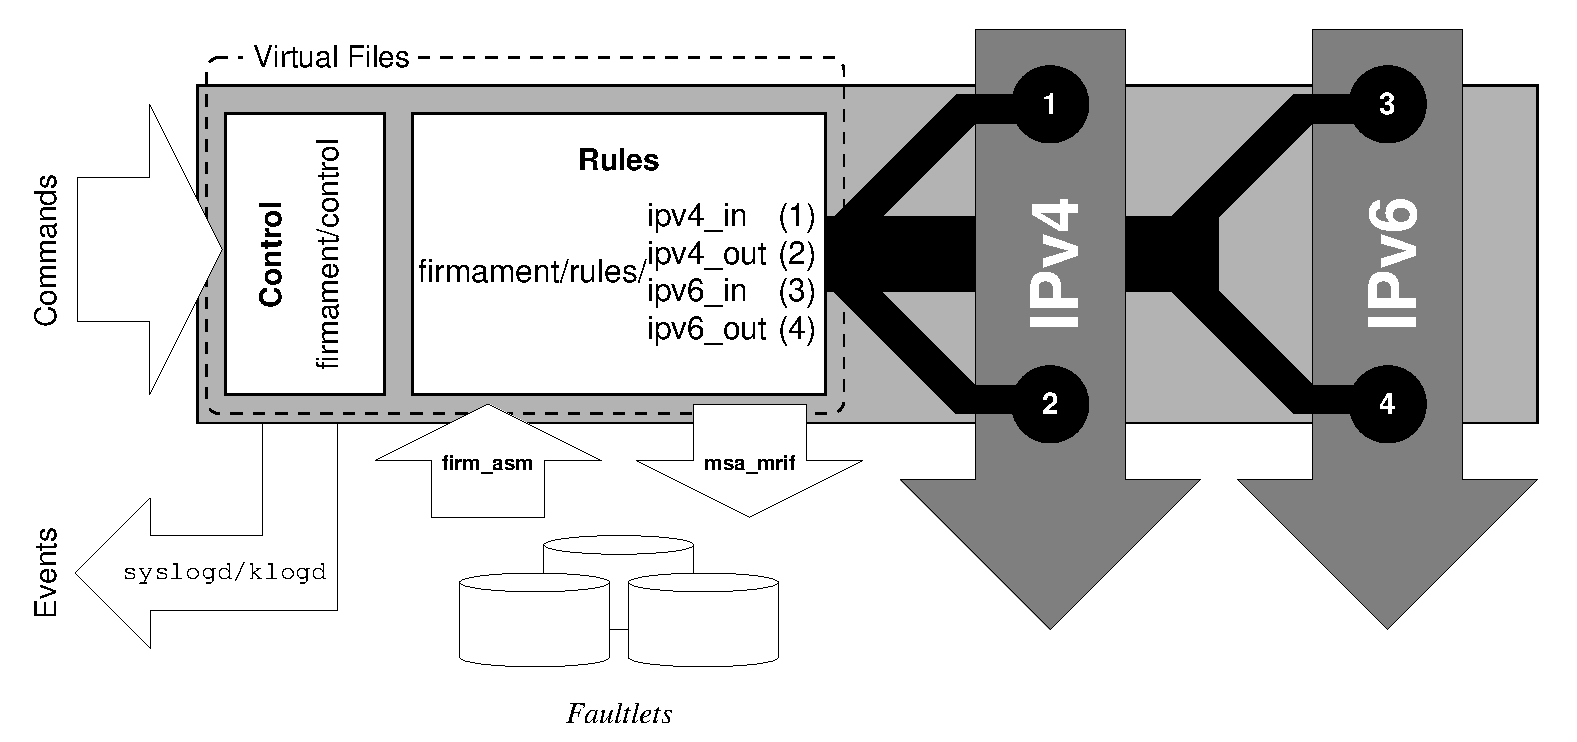
\includegraphics[width=.95\textwidth]{fig/architecture}
\caption{Conceptual relation of \textsf{FIRMAMENT}'s components}
\label{fig:arqfirm}
\end{figure}

\end{document}
